\section{Errors} \label{sec:errors}
In this section, we will present three types of errors which we implement in the simulation: path jitter, dephasing and data qubit displacement. Path jitter influences the probe qubit orbit (via the $r$-dependent interaction term in the Hamiltonian), whereas dephasing is introduced into the master equation through a Lindblad operator. Finally, we simulate data qubit displacement by adding a random offset for each of the four data qubits. In connection to qubit displacement, we will review a technique called \emph{twirling} which averages out the effect of displacement errors. Before we do so, however, we must first make explicit how we can quantify the performance of the system. 

\subsection{Benchmarking}
In our simulation, there are two significant ways to quantify errors, and we shall quickly review them here.

The first way is to look at the phase $\phi$ accumulated by the probe qubit through the interaction with the data qubits. In the proposal \citet{OGorman2016} a general phase jitter is introduced as a collective error for irregularities in the interaction. It is define as $\phi + \delta$, where $\delta$ is a small deviation from $\frac{\pi}{2}$.  Their simulations found that a phase jitter of $4.4 \%$ did not have a substantial impact on the fault-tolerance threshold. We will therefore attempt to compare the phase error in our simulation with this value whenever possible. %It should be noted, however, that the data we have access to usually concerns the entire run. We will therefore compare the phase error with $2\pi$ or $\pi$. We have made the assumption that the phase error for one quarter run stacks, such that after the full orbit the phase error of $\frac{\pi}{2}$ is the same percentage as the phase error of $2\pi$ that we observe. 

The second way to quantify errors is to look at the probability of correctly identifying the stabiliser state  $\ket{\psi}$ by measuring the probe qubit. As already mentioned, the outcome of the stabiliser measurement depends on whether we find $\ket{\psi}$ to be in the $\ket{+}$ or $\ket{-}$ state. The probability $p$ is given by $|\braket{+|\psi}|^2$ in the case of an even parity measurement and $|\braket{- |\psi}|^2$ in the case of an odd parity measurement. The need for this measure arises for example when we introduce a dephasing term in the Lindblad equation. A dephasing operator will not cause any phase error to appear since dephasing only decreases the magnitude of the Bloch vector, not its direction. Therefore, the probability $p_{\mathrm{succ}}$ of successfully identifying the stabiliser state becomes a good indicator of performance. It ranges from $p_{\mathrm{succ}} = 1$ when the probe qubit state is completely pure and without phase error to $p_{\mathrm{succ}} = 50 \%$ when the state has completely decohered and the stabiliser measurement becomes inherently random. %The probability of failure is subsequently given by $p_{\mathrm{f}} =1- p_{\mathrm{succ}}$, and this is the error that we will eventually compare with the probability of failure quoted for the surface code threshold. 

With these two measures in mind, let us look at the errors we introduced into the simulation and their effect on the performance of the system. 




%\clearpage
\subsection{Path jitter}\label{sec:jitter}
The first error that we shall introduce is a jitter present in the probe qubit orbit. The precision provided by modern MEMS control structures depends on the speed we want to operate them at \cite{Chu2003,Koo2012}. Improvements are needed to implement a $1\, $kHz operation (which corresponds to the expected parity measurement time) with near $1\, $nm precision but we expect improvements in the near future. Nevertheless, adding a random path jitter into the simulation will give us a good picture of what kind of phase error we can expect. At first, we attempted to simulate random jumps in the trajectory, but the discontinuities led to large derivative terms which in turn caused the simulation to fail. Thus,  we instead superposed a sinusoidal motion onto the trajectory path. To ensure an element of randomness in the motion, we varied the phase with which the sinusoidal motion starts. The amplitude of the motion represents the largest jitter errors on the scale of nanometres. The results can be found in fig.\@ \ref{fig:pathjitter}, where we note that an uncertainty of about 2 nm is sufficient for staying below the phase error threshold of $4.4 \%$.  It is sufficient to consider jitter in the $y$-direction instead of both the $x$ and $y$ directions, since the phase error is symmetric between them. 
From the graph it also becomes clear that jitter in the $z$-direction has the greatest influence. This is due to the $\frac{1}{r^3}$  term in the Hamiltonian.



\begin{figure}[h]
  \centering
    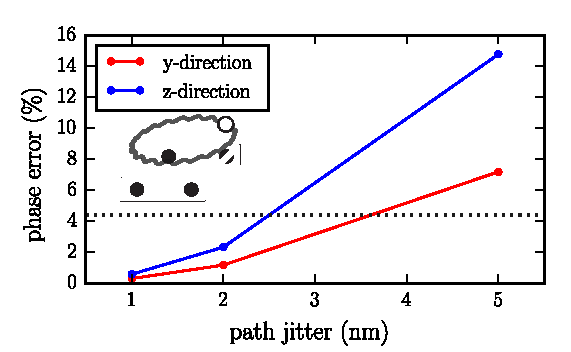
\includegraphics[width=0.5\textwidth]{../Figures/path_jit.pdf}
      \caption{Graph representing the percentage of phase error as a function of phase jitter in the $y$-direction (red) and in the $z$-direction (blue). There is a stronger dependence in the $z$-direction due to the $1/r^3$ term in the Hamiltonian.}
      \label{fig:pathjitter}
\end{figure}







\subsection{Dephasing}\label{sec:dephasing}
Next, we investigated the influence of dephasing on the measurement probabilities. In order to simulate dephasing, which is the gradual reduction of the Bloch vector in the $x$-$y$ plane towards the origin of the Bloch sphere, we introduced a Lindblad operator into the master equation. This operator is given by 
\begin{equation*}
L  = \sqrt{\Gamma} \sigma_z
\end{equation*}
where $\Gamma$ is the dephasing parameter, which can also be written as $1/T$ where $T$ is the dephasing time. In fig. \ref{FIG:abr-deph}, we show the effects of a dephasing time of $1.2\, $ms given an abrupt orbit, and in figure \ref{FIG:circ-deph} we show the effects of the same dephasing time of $1.2\, $ms for a circular orbit. In the latter case, the probe first sits far away from the data qubit, where the interaction is weak and the only evolution is due to the dephasing. Then as it moves closer, the interaction gets stronger very rapidly, causing the probe qubit to pick up a $\frac{\pi}{2}$ phase. Finally, as it moves away, the dephasing is again the dominant mechanism. 
It is clear that dephasing has a much more severe impact for the circular orbit, due to the increased amount of time required. 

\begin{figure}[H]
	\subfloat[]{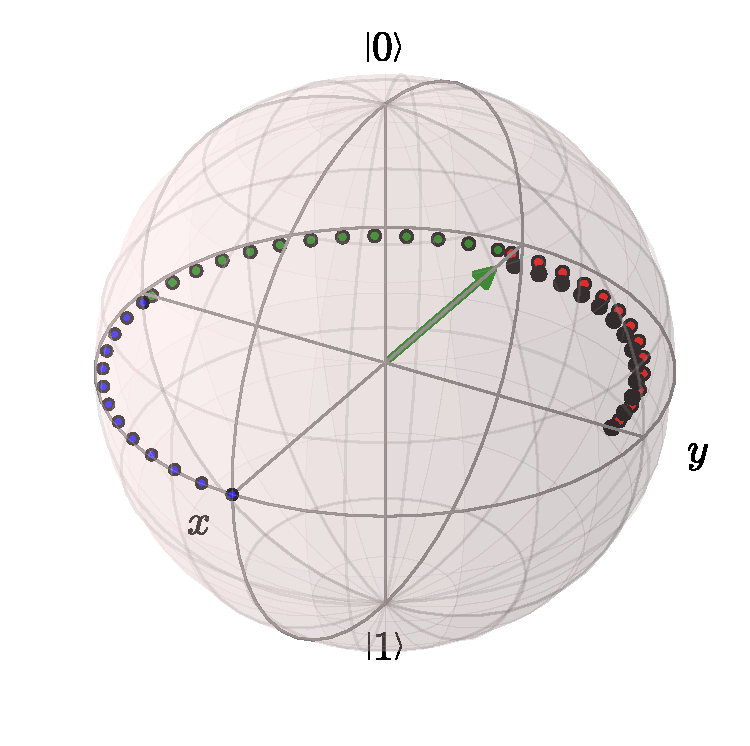
\includegraphics[width=0.49\linewidth]{../Figures/abrupt-deph} \label{FIG:abr-deph}} 
	\subfloat[]{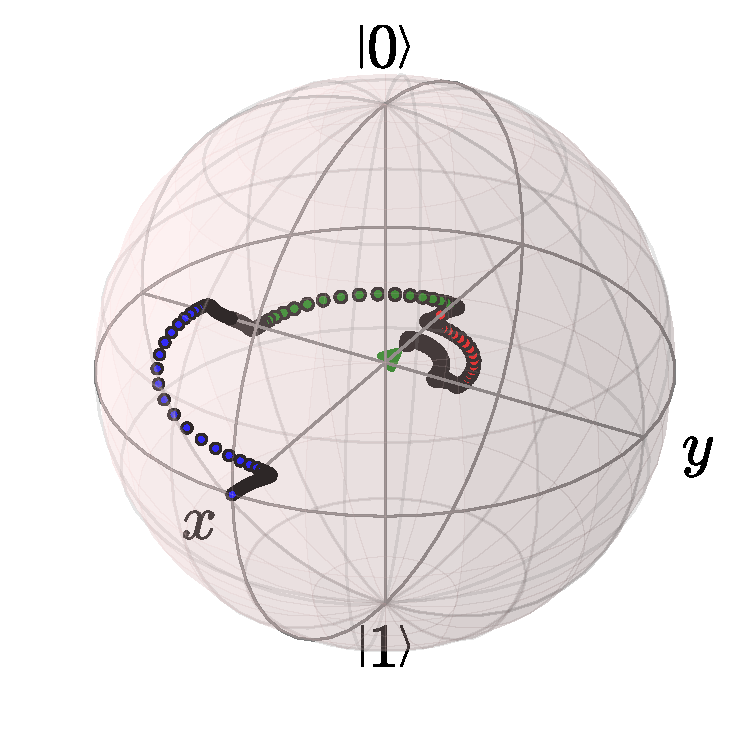
\includegraphics[width=0.49\linewidth]{../Figures/circ-deph} \label{FIG:circ-deph}}
	\caption[oddeven]{The evolution of the probe qubit state plotted in the Bloch sphere for a dephasing time $1.2\, $ms where one of the data qubits contains an error. The phase of the probe qubit is not affected since no relaxation or excitation is taking place. The effect can however be seen in the probability of measuring the probe qubit in the $\ket{+}$ or $\ket{-}$ state. \textbf{(a)} shows the dephasing for an abrupt orbit and \textbf{(b)} shows the dephasing for a circular orbit.}
	\label{FIG:deph}
\end{figure}


However, since dephasing does not affect the phase accumulated after the full run, we do not end up with a phase error. Therefore, the only accurate measure of errors due to dephasing is the measurement probability $p_{\mathrm{succ}}$. We ran simulations for both the abrupt and circular orbit using the $T_2$ and $T_2^*$ values given in table\@ \ref{TAB:qubits} as input parameters for the dephasing time. The results are shown in fig.\@ \ref{fig:dephasingplot}, where each data point refers to an entry in the table. 

We can compare the probability of correctly measuring the stabiliser in the $\ket{-}$ state with the surface code fault-tolerance threshold of $1.1\%$, which translates into a success probability of $98.9$\%. Looking at the values displayed in fig.\@ \ref{fig:dephasingplot}, we find that only the clock transition in bismuth leaves us within the fault-tolerance threshold. For the circular orbit, bismuth $(1)$ has a success probability of  99.9\% after one entire run. The next best value is obtained for NV centres at room temperature $(2)$ which give us a success probability of 57.7\% in the case for the circular orbit, and 92.1\% for the abrupt orbit. Both of these probabilities are outside the surface code threshold. 

We see that the clock transition in bismuth does exceptionally well, but that many spin species decohere long before the run is complete. This is especially clear in the case for the circular orbit, which takes approximately $10$ times longer than the abrupt orbit. It should be noted however that our results for the $T_2^*$ time (representing reversible loss of coherence) assume that no measures of refocusing, such as Hahn echoes \cite{levitt1979nmr} or dynamical decoupling \cite{viola1998dynamical} are taken. Note that any echo technique would have to be applied on both the probe qubit and the data qubit to preserve the direction of the evolution. 

As we discuss in more detail in Section \ref{sec:conclusions}, the impact of dephasing could be decreased by lowering the time needed for the probe qubit to complete one orbit around the data qubits. This would require lowering the distance $d$ between the probe qubits and the data qubits as to increase the interaction strength between them. 





\begin{figure}[h]
	\centering
	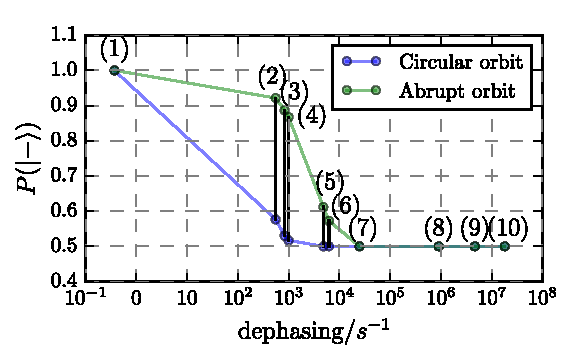
\includegraphics[width=1.05\linewidth]{../Figures/dephasing.pdf}
		\caption{A graph showing the relationship between the dephasing parameter $\Gamma$ and the probability $P(\ket{-})$ of measuring the probe qubit in the $\ket{-}$ state.  The blue data points represent an abrupt orbit and the green data points a circular orbit. Each number refers to a dephasing time found in table\@ \ref{TAB:qubits}. }
		\label{fig:dephasingplot}
\end{figure}





